In this section we present our causal estimand, identifying assumptions, estimation strategy, and inferential procedure.

\subsection{Estimand}

Our goal is to estimate the average effect 2014 Medicaid expansion would have had on the non-elderly adult uninsurance rate in states that did not expand Medicaid. Let $A$ indicate treatment assignment, $c$ index a CPUMA, $s$ index the state, and $t$ index the time period. Let $n_1$ be the number of treated CPUMAs, $n_0$ be the number of control CPUMAs, and $n$ be the total number of CPUMAs. Similarly, let and $m = m_1 + m_0$ states (with $m_1$ and $m_0$ defined analogously). Each state has $p_s$ CPUMAs. $A_s=0$ indicates untreated states and $A_s=1$ indicates treated states, when this notation is a superscript if it indicates the potential outcome. Since we are only interested in the counterfactual at time $T = 2014$, we simplify notation by removing this variable and the subscript and write our formal estimand as:

\begin{equation}
\psi = \psi^1 - \psi^0 &= n_0^{-1}\sum_{s, c: A_s = 0} Y_{sc}^{A_s = 1} - Y_{sc}^{A_s = 0} 
\end{equation}

The challenge is that we do not observe the counterfactual outcomes for non-expansion CPUMAs had they been in states that expanded their Medicaid programs. We therefore require causal assumptions to tie this counterfactual quantity to our observed data.\footnote{The 2014 Medicaid expansion occurred simultaneously with the implementation of several other major ACA provisions, including (but not limited to) the creation of the ACA-marketplace exchanges, the individual mandate, health insurance subsidies, and community-rating and guaranteed issue of insurance plans (\cite{courtemanche2017early}). Almost all states broadly implemented these reforms beginning January 2014. Conceptually we think of the other ACA components as a state-level treatment ($R$) separate from Medicaid expansion ($A$). Therefore, our total estimated effect may also include interactions between these policy changes; however, we do not attempt to separately identify these effects. Because the ACA implementation and Medicaid expansion may vary over time, we do not try to generalize these results beyond 2014.} 

\subsection{Identification}

The following causal assumptions are necessary (though insufficient) to identify our target parameter from our observed data: the stable unit treatment value assumption (SUTVA), no unmeasured confounding, and no anticipatory treatment effects. We explain these assumptions in detail and their consequences below. We additionally invoke several parametric assumptions to help us identify our causal parameter given the measurement error in our covariates. These assumptions in total are sufficient to identify our causal estimand.

SUTVA has two implications: first, that there is only one version of treatment; second, that $Y_{sc}^{\mathbf{a}} = Y_{sc}^{\mathbf{a}'}$ when $a_{sc} = a_{sc}'$, where $\mathbf{a}$ is the vector of all treatment assignments. We discussed potential violations of the first assumption previously when considering how to reduce Medicaid Expansion to a binary treatment classification. Our solution is to remove states with less restrictive Medicaid eligibility requirements prior to 2014 to approximately satisfy this condition. The second part of this assumption implies that the potential outcomes in each region do not depend on another region's treatment assignment. This is a standard assumption, but is often not realistic in practice. Violations are likely in our setting: for example, \cite{frean2017premium} find evidence that Medicaid expansion drove previously eligible but uninsured individuals to enroll in Medicaid in both expansion and non-expansion states. Signing the potential bias from this violation requires redefining the causal estimand: for example, we might consider the treatment effect on the untreated given that all states have expanded Medicaid, where the contrast is against where only the observed expansion states expanded Medicaid. If the spillover effects were equal in each region, and the magnitude of the spillovers increase with the total number of treated regions, then the true effect would be larger in absolute magnitude than the estimated effect using the observed data. We could consider other estimands or assumptions to get different predictions about the sign of the bias; however, this is beyond the scope of this paper.

We next assume that there were no anticipatory treatment effects. Letting treatment occur at time $T$, we have that for $t < T$:

\begin{align*}
Y_{sct} = Y_{sct}^0
\end{align*}

This assumption is necessary because we will condition on pre-treatment outcomes. If these outcomes were affected by the treatment before it were implemented, these covariates would be endogenous. Anticipatory treatment effects may occur if plans to expand Medicaid induce uninsured but Medicaid-eligible individuals to enroll in Medicaid prior to expansion. We do not think these violations occurred in large enough numbers to substantially affect our results. Instead, we address a more concerning version of this violation: the fact that several states allowed certain counties to expand Medicaid prior to 2014. We test the sensitivity of our results to the exclusion of these states.

Third, we assume no unmeasured confounding; that is, that at time $T$ the potential outcomes for each CPUMA are independent of the state-level treatment assignment conditional on the population-level CPUMA and state-level covariates $X_{sc}$, a $q$ dimensional vector of covariates (which includes pre-treatment outcomes):

\begin{align*}
Y_{sc}^a \perp A_{sc} \mid X_{sc}
\end{align*}

While unverifiable, we believe it is reasonable here given our rich covariate set. To be explicit, we believe that the pair of potential uninsurance rates for each CPUMA are independent of the treatment assignment conditional on the percentage of uninsured individuals in each year of the pre-treatment period, the percentage of unemployed individuals in each year of the pre-treatment period, the average population growth, the average ratio of households to non-elderly adult population, the state's political composition, the average proportion of households with one, two, or three or more children during the pre-treatment period, the average proportion of households who did not respond about their number children, and the average proportion of individuals during the pre-treatment period with given demographics noted above (age group, sex, white, Hispanic ethnicity, U.S. citizenship, foreign born, income-to-poverty group (including non-response), disability status, urban residence, and educational attainment group). 

A key problem we address in this paper is the violation of this assumption due to measurement error in our covariates. Let 
$X = (X_0, X_1)^T$ be the $n$ by $q$ matrix of true covariates (and separating the control from treated units using $X_a$). Because our covariates are estimated using the ACS data, rather than $(Y, X)$, we instead observe $(J,W)$, which consist of estimates of the true outcome and covariate values, where $W$ is structured analogously to $X$. Importantly, $Y_{sc}^a \perp A_{sc} \mid X_{sc} \centernot\implies J_{sc}^a \perp A_{sc} \mid W_{sc}$. The use of these proxies may therefore bias our estimates. We rely on several modeling assumptions to correct for this.

We first model our observed data as functions of the true values plus mean-zero Gaussian noise: $J_{sc} = Y_{sc} + \xi_{sc}$ and $W_{sc} = X_{sc} + v_{sc}$, where we assume $\xi_{sc}$ and $v_{sc}$ are independent though not identically distributed.\footnote{Our covariates are almost all ratio estimates, which will in general be biased. This bias, however, decreases quickly with the sample size (is $O(n^{-1})$). Given that our CPUMA sample sizes are all over 300, we treat these estimates as unbiased in our analysis.} We assume that these errors are uncorrelated with the true values, i.e. $\mathbb{E}\{\xi_{sc} \mid Y_{sc}\} = 0$ (and similarly for all elements of $X$). Second, we assume that $\xi_{sc}$ are uncorrelated with the errors in the covariate measurements. These assumptions and our model for the observed data are reasonable given that the measurement error in this context is sampling variability. Moreover, our outcomes are measured on a different cross-section than our covariates, so it is reasonable to assume that they are uncorrelated with the measurement errors in the covariates. 

We next assume that the true potential outcomes are linear in the true covariates $X_{sc}$. Specifically, we assume that the following model generates the potential non-elderly adult uninsurance rate under treatment $A = a$:

\begin{equation}\label{eqn:outcomemodel}
Y_{sc}^a = \alpha_a + X_{sc}^T\beta_a + \epsilon_{sc} + c_s
\end{equation}

We assume that the errors $\epsilon_{sc}$ and $c_s$ are mean-zero, independent from each other and across time (i.e., we rule out serial-correlation), and are uncorrelated with the true covariates and the treatment assignment, i.e. $\mathbb{E}\{\epsilon_{sc}c_s \mid X_{sc}, A_s\} = \mathbb{E}\{\epsilon_{sc} \mid X_{sc}, A_s\} = \mathbb{E}\{c_s \mid X_{sc}, A_s\} = 0$. We can then identify $\psi^a$ in terms of our model parameters (see Appendix A); specifically, we have that $\psi^a = \alpha_a + \bar{X}_0^T\beta_a$, where $\bar{X}_0$ is the vector of mean covariate values among the control units. Moreover, we can substitute $J_{sc}$ for $Y_{sc}$ in Equation~\ref{eqn:outcomemodel}, and add $\xi_{sc}$ to the error term without affecting identification. 

We still have the problem that we observe $W_{sc}$ instead of $X_{sc}$. Let $\eta_a = \mathbb{E}\{X_{sc} \mid W_{sc}, A_s = a\}$. By linearity, we know that

\begin{equation}
    J_{sc} = \eta_a(W_{sc})^T\beta + (X_{sc} - \eta_a(W_{sc}))^T\beta + \xi_{sc} + \epsilon_{sc} + c_s 
\end{equation}

If we knew $\eta_a$, we could estimate this model using the observed data $(J, W)$. The approach we follow here is known as ``regression calibration'' in the measurement-error literature. In particular, we assume a linear model for $\eta_a$:

\begin{align*}
\eta_a(W_{sc}) = \upsilon_a + \kappa_a^T(W_{sc} - \upsilon_a)
\end{align*}

where $\kappa_a = (\Sigma_{XX \mid A = a} + \Sigma_{vv \mid A = a})^{-1}\Sigma_{XX \mid A = a}$. The assumption motivating this model is that $(X_{sc}, v_{sc}) \stackrel{iid}\sim MVN((\upsilon_a, 0), \Sigma_a)$ and $\Sigma_a$ is a $2q$ by $2q$ block-diagonal matrix consisting of $q$ by $q$ matrices $\Sigma_{XX \mid A = a}$ and $\Sigma_{vv \mid A = a}$ and $0$ in the off-diagonals. Given sufficient auxillary data to estimate $\kappa_a$, we can then estimate $\psi$. We discuss this further below and in Appendices A and B (see also \cite{gleser1992importance}).

\subsection{Estimation}

We outline our estimation strategy first emphasizing how estimating the ETC differs from estimating the ETT with respect to variable selection under the ``synthetic controls'' framework and associated assumptions required. Second, we explain our estimation procedure, which modifies the SBW criterion to address the hierarchical data structure. This objective, which we call H-SBW, reduces the variance of our estimator under our assumption of constant variance and constant within-state correlation of model errors. Third, we connect our estimator to the regression calibration literature by generating weights that balance a linear prediction of the true covariates $\hat{\eta}_a(W_{sc})$ using the observed covariates $W_{sc}$. Fourth, we test the sensitivity of our estimator to a regression-augmented version, using ridge-regression weights following the suggestion of \cite{ben2018augmented}; this allows us to achieve better covariate balance by extrapolating beyond the support of the data. We conclude by proposing a model validation procedure that uses pre-treatment outcomes to compare the performance of our estimators on pre-treatment data.

\subsubsection{Variable selection}

We seek to generate a set of positive weights that balance the means of covariates for the treated units to the mean covariates for the control units. Assume that we observe the true covariate matrices for the treated data $X_a = (X_{a,1}, ..., X_{a, q})$, and the true outcomes $Y$. Let $\bar{X}_{0, r}$ be the mean covariate value for the $r$-th covariate in the non-expansion region. Ideally, there exists some $\gamma^\star \in \Gamma$ satisfying: 

\begin{equation}\label{eqn:constraint}
\Gamma = \{\gamma \in \mathbb{R}^{n_1}: &\lvert \gamma^TX_{1, r} - \bar{X}_{0, r} \lvert \le \delta_r \ \ (r = 1, ..., q), \ \gamma_{sc} > 0, \sum_{s, c: A_{sc} = 1}\gamma_{sc} = 1\}
\end{equation}

for $\delta_r = 0$ for all $r = 1, ..., q$. We could then estimate $\psi$ as

\begin{equation}\label{eqn:psi}
\hat{\psi} = \sum_{s: A_s = 1}^{m_1}\sum_{c = 1}^{p_s}\gamma_{sc}^\star Y_{sc} - n_0^{-1}\sum_{s: A_s = 0}^{m_0}\sum_{c = 1}^{p_s}Y_{sc}
\end{equation}

Again assuming that the potential outcomes are a linear function of the true covariates: $\mu_a(X_{sc}) = \alpha_a + X_{sc}^T\beta_a$, the bias of our estimate of $\psi^1$ (again assuming we observed $X_{sc}$), is less than or equal to $\lvert\beta_1\rvert^T\delta = 0$ (see, e.g., \cite{zubizarreta2015stable}). The challenge is that for any given dataset we have no guarantee that any such $\gamma^\star$ exists that exactly balances the covariates. We therefore often require some method of determining which parts of the covariate distribution we wish to prioritize balancing - or which covariates to balance at all - to minimize this bias.

The synthetic controls approach chooses the $\gamma$ that minimizes the weighted L2-squared distance of the covariates using a diagonal weighting matrix $V$. $V$ is then chosen to minimize the mean-square error of the weighted difference in pre-treatment outcomes. Letting $Z_a$ be the matrix of pre-treatment outcomes for treatment group $A = a$, the synthetic controls algorithm solves the following optimization problem for a fixed $V$:

\begin{align}
\gamma(V) = \arg\min_{\tilde{\gamma}(V^\star)} = (\bar{X}_1 - X_0^T\tilde{\gamma})'V(\bar{X}_1 - X_0^T\tilde{\gamma}) 
\end{align}

This is the ``inner'' optimization. $V^\star$ is then determined in an ``outer'' optimization to minimize the imbalances in the pre-treatment outcomes $Z$:

\begin{align}
    V^\star = \arg\min_V (\bar{Z}_1 - Z_0^T\gamma(V))'(\bar{Z}_1 - Z_0^T\gamma(V))
\end{align}

In applications the covariate matrix $X_a$ may contain some elements of $Z_a$. In cases where $X_a$ contains all pre-treatment outcomes, \cite{kaul2015synthetic} has shown that the predictor weights $V^\star$ will give no weight to auxillary covariates (covariates that are not the pre-treatment outcomes). 

While in practice $V$ is often learned on the same data as the weights, we consider the case where we use cross-validation to choose $V$, as proposed by \cite{abadie2015comparative}. Assume we can divide our pre-treatment data into a training data from periods $T = 1, ..., T - l - 1$, a validation period from periods $T - l, ..., T - 1$, and a post-treatment period at time $T$. To make this discussion more general, assume that we are evaluating a set of $\mathcal{M}$ candidate models on the validation data (where for the synthetic controls algorithm we can think of this as the set of all possible weighting matrices $V$). Let $\bar{Y}^a_{a', t}$ be the mean potential outcome under treatment $A = a$ for treatment group $A = a'$ at time $t$ (where $t$ occurs during the validation period). Let $\hat{\bar{Y}}^a_{a'', t}(m)$ be an estimator of that potential outcome at time $t$ using model $m$, which was trained during the training period using data from treatment group $A = a''$. Finally, let $\bar{Y}_{a'}^a_T$ be the post-treatment estimand, where $\hat{Y}^a_{a'', T}(m)$ is the estimator using model $m$ trained using validation period data. This learning procedure implicitly assumes that:

\begin{align*}
m^\star = \min_{m \in \mathcal{M}}\sum_{T - l}^{T-1}\|\hat{Y}^0_{0, t}(m) - \bar{Y}^0_{1, t}\| = \min_{m \in \mathcal{M}}\mathbb{E}\{\|\hat{Y}^0_{0, T}(m) - \bar{Y}^0_{1, T}(m)\|\}
\end{align*}

In other words, we select our model using the empirical loss in the validation period as a proxy for the expected loss in the post-treatment time-period.\footnote{It is possible that multiple models in $\mathcal{M}$ either perfectly predict the pre-treatment outcomes, or predict them equally well. In this case we would require an additional criteria to choose the optimal model (see, e.g, \cite{becker2017cross}}. This makes intuitive sense in the typical synthetic controls setting where the estimand is the ETT since we observe $Y^0_{sct}$ for $t < T$. When synthetic controls are used to estimate the ETC, this strategy alone is insufficient as we never observe $Y^1_{sct}$ (or a mean-unbiased proxy) prior to treatment for any unit. We therefore cannot easily use pre-treatment outcomes to optimally select variables or determine relative covariate importance without stronger assumptions.

One such assumption is the following:

\begin{align}\label{assumption:second}
m^\star = \min_{m \in \mathcal{M}}\sum_{T - l}^{T-1}\|\hat{Y}^0_{1, t}(m) - \hat{Y}^0_{0, t}\| = \min_{m \in \mathcal{M}}\mathbb{E}\{\|\hat{Y}^1_{1, T}(m) - \bar{Y}^1_{0, T}\|\}
\end{align}

We call this assumption ``counterfactual risk invariance.'' In other words, we assume that the model that minimizes the validation-period risk also minimizes the post-treatment risk. This is a very strong assumption for conducting any form of variable selection or covariate weighting in this setting. As a simple example, assume that we can partition $X = (R, S)$, where, for simplicity, we assume $S$ is univariate. Further assume that $Y^0_t \perp A \mid R$ for all $t = 1, ..., T$ but that $Y^1_T \perp A \mid X$. Again assume that $\mu_a$ are linear in the covariates with (time-invariant) coefficients $\beta_{a, r}$ ($r = 1, ..., q$). These assumptions imply that $\beta_{0, s} = 0$. If our goal is to predict the ETT, then we wish to use the untreated data to predict $\bar{Y}_{1, T}^0$. We may then conduct some variable selection procedure using our pre-treatment data, learn that covariate $S$ is unimportant, and estimate a model that downweights imabalances in $S$ (or ignores the covariate entirely) but perfectly balances the remaining covariates. This model would give an unbiased estimate of the counterfactual outcome for the treated group absent treatment in time-period $T$. However, if our goal were instead to predict $\bar{Y}^1_{0, T}$ -- the counterfactual outcome under treatment for the untreated units -- the same procedure applied to the treated data would again downweight $S$ and result in a biased estimate, with bias equal to $(\gamma^TS_1 - \bar{S}_0) \beta_{1, s}$. If $S$ is a strong predictor of treatment assignment, this could lead to substantial bias. \footnote{We conflate two issues in this discussion: the synthetic controls variable weighting algorithm and variable selection more generally. Provided $S$ is contained in $X$ and exact balancing weights exist with high probability as $n \to \infty$, then under our modeling assumptions, the synthetic controls procedure is still consistent for $\psi^1$ even if the variable weights $V$ are sub-optimal. However, if covariates $S$ are not contained in $X$ at all, then this procedure will not balance these covariates even asymptotically provided that $\mathbb{E}\{S \mid A = 1\} \ne \mathbb{E}\{S \mid A = 0\}$. However, here we take a finite-sample perspective. Imbalances in $S$ will lead to bias, whether or not $S$ is imbalanced due to receiving low weights on the weighting matrix $V$, or omitted from the objective entirely.} 

As a practical example, we highlight the potential confounding role of Republican governance for our counterfactual estimate. Republican governance is a strong predictor of a state's decision to expand Medicaid \cite{courtemanche2017early}. Moreover, existing evidence prior to Medicaid expansion showed that Medicaid take-up rates were lower in more conservative states \cite{sommers2012understanding}. Yet when generating their synthetic control weights to estimate the ETT, \cite{courtemanche2017early} and \cite{kaestner2017effects} do not control for these factors. \footnote{\cite{courtemanche2017early} does control for Republican governor in their regression model and they find that it is a statistically significant predictor of 2013 uninsurance rates. One reason they may not control for this in the synthetic control model is practical: it is much harder to balance this covariate using control data without extrapolating from the data.} However, it is clear that if take-up rates depend on governance, we may expect this to be a strong confounder of $Y^1$ and hence confound the ETC, even if arguably it is not a confounder of $Y^0$ (and hence not a confounder for the ETT).

We demonstrate this in our application by conducting a variable importance analysis. Specifically, we remove the balance constraints from the Republican governance indicators and examine how our estimates of $\hat{\psi}^1$ change. Letting $\hat{\psi}^1_s$ be the estimate when removing the Republican governance indicators (or more generally, the covariate matrix $S$ where $X = (R, S)$). We subtract our original point estimate $\hat{\psi}^1_0$ from $\hat{\psi}^1_s$ to generate the difference $\hat{\Delta}^1$. This difference tells us about the direction of the bias our estimate of $\hat{\psi}^1$ would incur when we do attempt to constrain the imbalance in covariate $S$. Our hypothesis implies that we should expect $\hat{\Delta}_s^1 < 0$: that is, keeping all other covariates (roughly) fixed, we expect the predicted uninsurance rate will decrease when as the level of Republican governance decreases. In addition to the Republican governance indicators, we also examine four other covariate groups: pre-treatment uninsurance rates and pre-treatment unemployment rates, and three sets of different demographic indicators, which we detail in Appendix E.\footnote{We caution that our results do not imply that Republican governance is not an important confounder of $Y^0_{1, T}$ since we do not analyze this directly.} 

Overall we emphasize that predicting the outcome under treatment is different, and perhaps more challenging, than predicting the outcome absent treatment. The former requires understanding which covariates matter most to predicting treatment response, which we cannot as naturally learn from pre-treatment outcomes. We instead rely on our prior knowledge and modeling assumptions to choose which covariates to balance and which covariates to prioritize in this balancing. We point out that modeling the ETC requires greater justification of the covariates used to predict treatment response than for the ETT, and that using the standard synthetic controls variable weighting procedure is unlikely to be optimal for this purpose.\footnote{Our analysis assumes no unmeasured confounding and a linear model for $\mu_a$. By contrast, synthetic controls are frequently motivated by a linear factor model for $\mu_0$. \cite{abadie2010synthetic} and \cite{ferman2016revisiting} outline conditions where this method is consistent as the number of pre-treatment outcomes goes to infinity, in particular because the method balances the unobserved factor loadings. Analogous to our analysis, if we assume $\mu_{a, T}$ both follow a linear factor model, identification of the ETC requires that the factors that confound $Y^1_T$ are the same that confound $Y^0_t$. Under this assumption, we might be able to show that the synthetic control estimator is consistent in this setting. However, the tuning procedure to determine the predictor weights may again be sub-optimal from a finite-sample bias perspective, depending again on how the covariates (or unobserved factors) that are most predictive of treatment response vary between treatment groups and on their associations with the potential outcomes.}

Given these challenges, we therefore use a variation of SBW to estimate the ETC.\footnote{Specifically, we use a modified implementation of Noah Griefer's ``optweight'' package in R, available on github.com/mrubinst757} SBW minimizes the variance of the weights subject to user-specified balance constraints. The primary advantages of H-SBW over synthetic controls in this setting are that it gives the user finer control over the desired levels of covariate balance, allowing the user to navigate a bias-variance tradeoff with respect to balance and the variability of the weights. Specifically, SBW weights solve the following minimization:

\begin{equation}
\gamma &= \arg\min_{\tilde{\gamma} \in \Gamma} \quad \sum_{s: A_s = 1}^{m_1}\sum_{c = 1}^{p_s} \tilde{\gamma}_{sc}^2  
\end{equation}

where $\Gamma$ is defined in Equation~\ref{eqn:constraint}. We can then estimate $\psi$ using Equation~\ref{eqn:psi}, substituting $J_{sc}$ for $Y_{sc}$ and plugging in the weights $\gamma$. By contrast, the synthetic controls algorithm will minimize the weighted L2 distance between the treated and control units in the criterion; this algorithm in general may lead to lower imbalances, but the balance tradeoffs are difficult to control, and the resulting weights may be more extreme. Finally, the algorithm, as formulated in \cite{abadie2010synthetic} and presented above, may not have a unique solution (but see \cite{ben2018augmented}, \cite{becker2017cross}).

For our primary estimates we lean heavily on assumptions to justify our choice of $\delta$. We use a priori domain knowledge about which covariates are most likely to be important predictors of treatment response when setting $\delta$, but also choose $\delta$ to avoid generating overly extreme weights. For our application, we constrain $\delta$ to be 0.05 percentage points (out of 100) for pre-treatment outcomes, 0.15 percentage points for pre-treatment unemployment rates, and 25 percentage points for the Republican governance indicators. We believe these covariates are most likely to predict treatment response. While we believe that Republican governance is an important covariate to balance, we are unable to reduce the constraints further given the support of the data. For the remaining covariates, we let $\delta$ be 0.5 percentage points for average population growth and household to adult ratio, 1 percentage point for female, Hispanic ethnicity, white race, age category, disability, and number of children category; 2 percentage points for urban, citizenship, education category, income-to-poverty category, student, and foreign-born, again choosing these constraints with respect to both feasibility and extreme weight concerns. 

\subsubsection{H-SBW objective}

The motivation of the SBW criterion is to produce the minimum variance weights for a fixed $\delta$. This produces the minimum variance estimator within the constraint set if, for example, the errors in the outcome model are independent and identically distributed \cite{zubizarreta2015stable}. In our setting we allow for possible state-level dependencies, potentially reducing the efficiency of the SBW estimator. To address this possibility, we add the tuning parameter $\rho \in [0, 1)$ in the objective below. Assuming a constant variance across units for each error component, $\rho$ represents a constant (and known) within-state correlation of the errors. 

\begin{equation}\label{eqn:objective}
\gamma &= \arg\min_{\tilde{\gamma} \in \Gamma} \quad \sum_{s: A_s = 1}^{m_1}(\sum_{c = 1}^{p_s} \tilde{\gamma}_{sc}^2 + \sum_{c \ne d}\rho \tilde{\gamma}_{sc}\tilde{\gamma}_{sd})\\
\end{equation}

For $\delta \to \infty$, this objective yields the solution:

\begin{equation}\label{eqn:sbwsol}
\gamma_{sc} \propto \frac{1}{(p_s - 1)\rho + 1}
\end{equation}

Setting $\rho \approx 1$, the solution becomes

\begin{equation}\label{eqn:sbwsol}
\gamma_{sc} \propto \frac{1}{p_s}
\end{equation}

In other words, this objective will attempt to downweight CPUMAs in states with large numbers of CPUMAs, upweight CPUMAs in states with small numbers of CPUMAs, and assign each CPUMA within a state equal weight. Notice that when $p_s$ is constant across states this objective returns the SBW solution when $\delta \to \infty$, and that SBW is equivalent to setting $\rho = 0$. In short, as we increase $\rho$, the objective will attempt to more uniformly disperse the weights across states. 

As a brief illustration, we simulate $N = 800$ observations in $m = 40$ regions each with $p_s = 20$ units, and draw $X_{sc} \sim N(\mu_s, 1)$, for $\mu \in \{0, 1\}$ (drawn from a Bernoulli with equal probability); $A_s \sim Bern(expit(\bar{X}_s))$. We then generate weights to balance the control to the treated group mean. We run H-SBW variants setting $\rho = 0$ (which is equivalent to SBW), $\rho = 0.5$, and $\rho = 0.99$ all while keeping $\delta$ fixed at zero. Figure 1 shows the weights summed to the group level for all control regions. The color of each set of bars is the overall variance of the weights. We can see that the weights in general are uniform across units for SBW, but poorly dispersed across regions, while the weights are more uniformly dispersed as we increase $\rho$. 

\begin{figure}
\begin{center}
    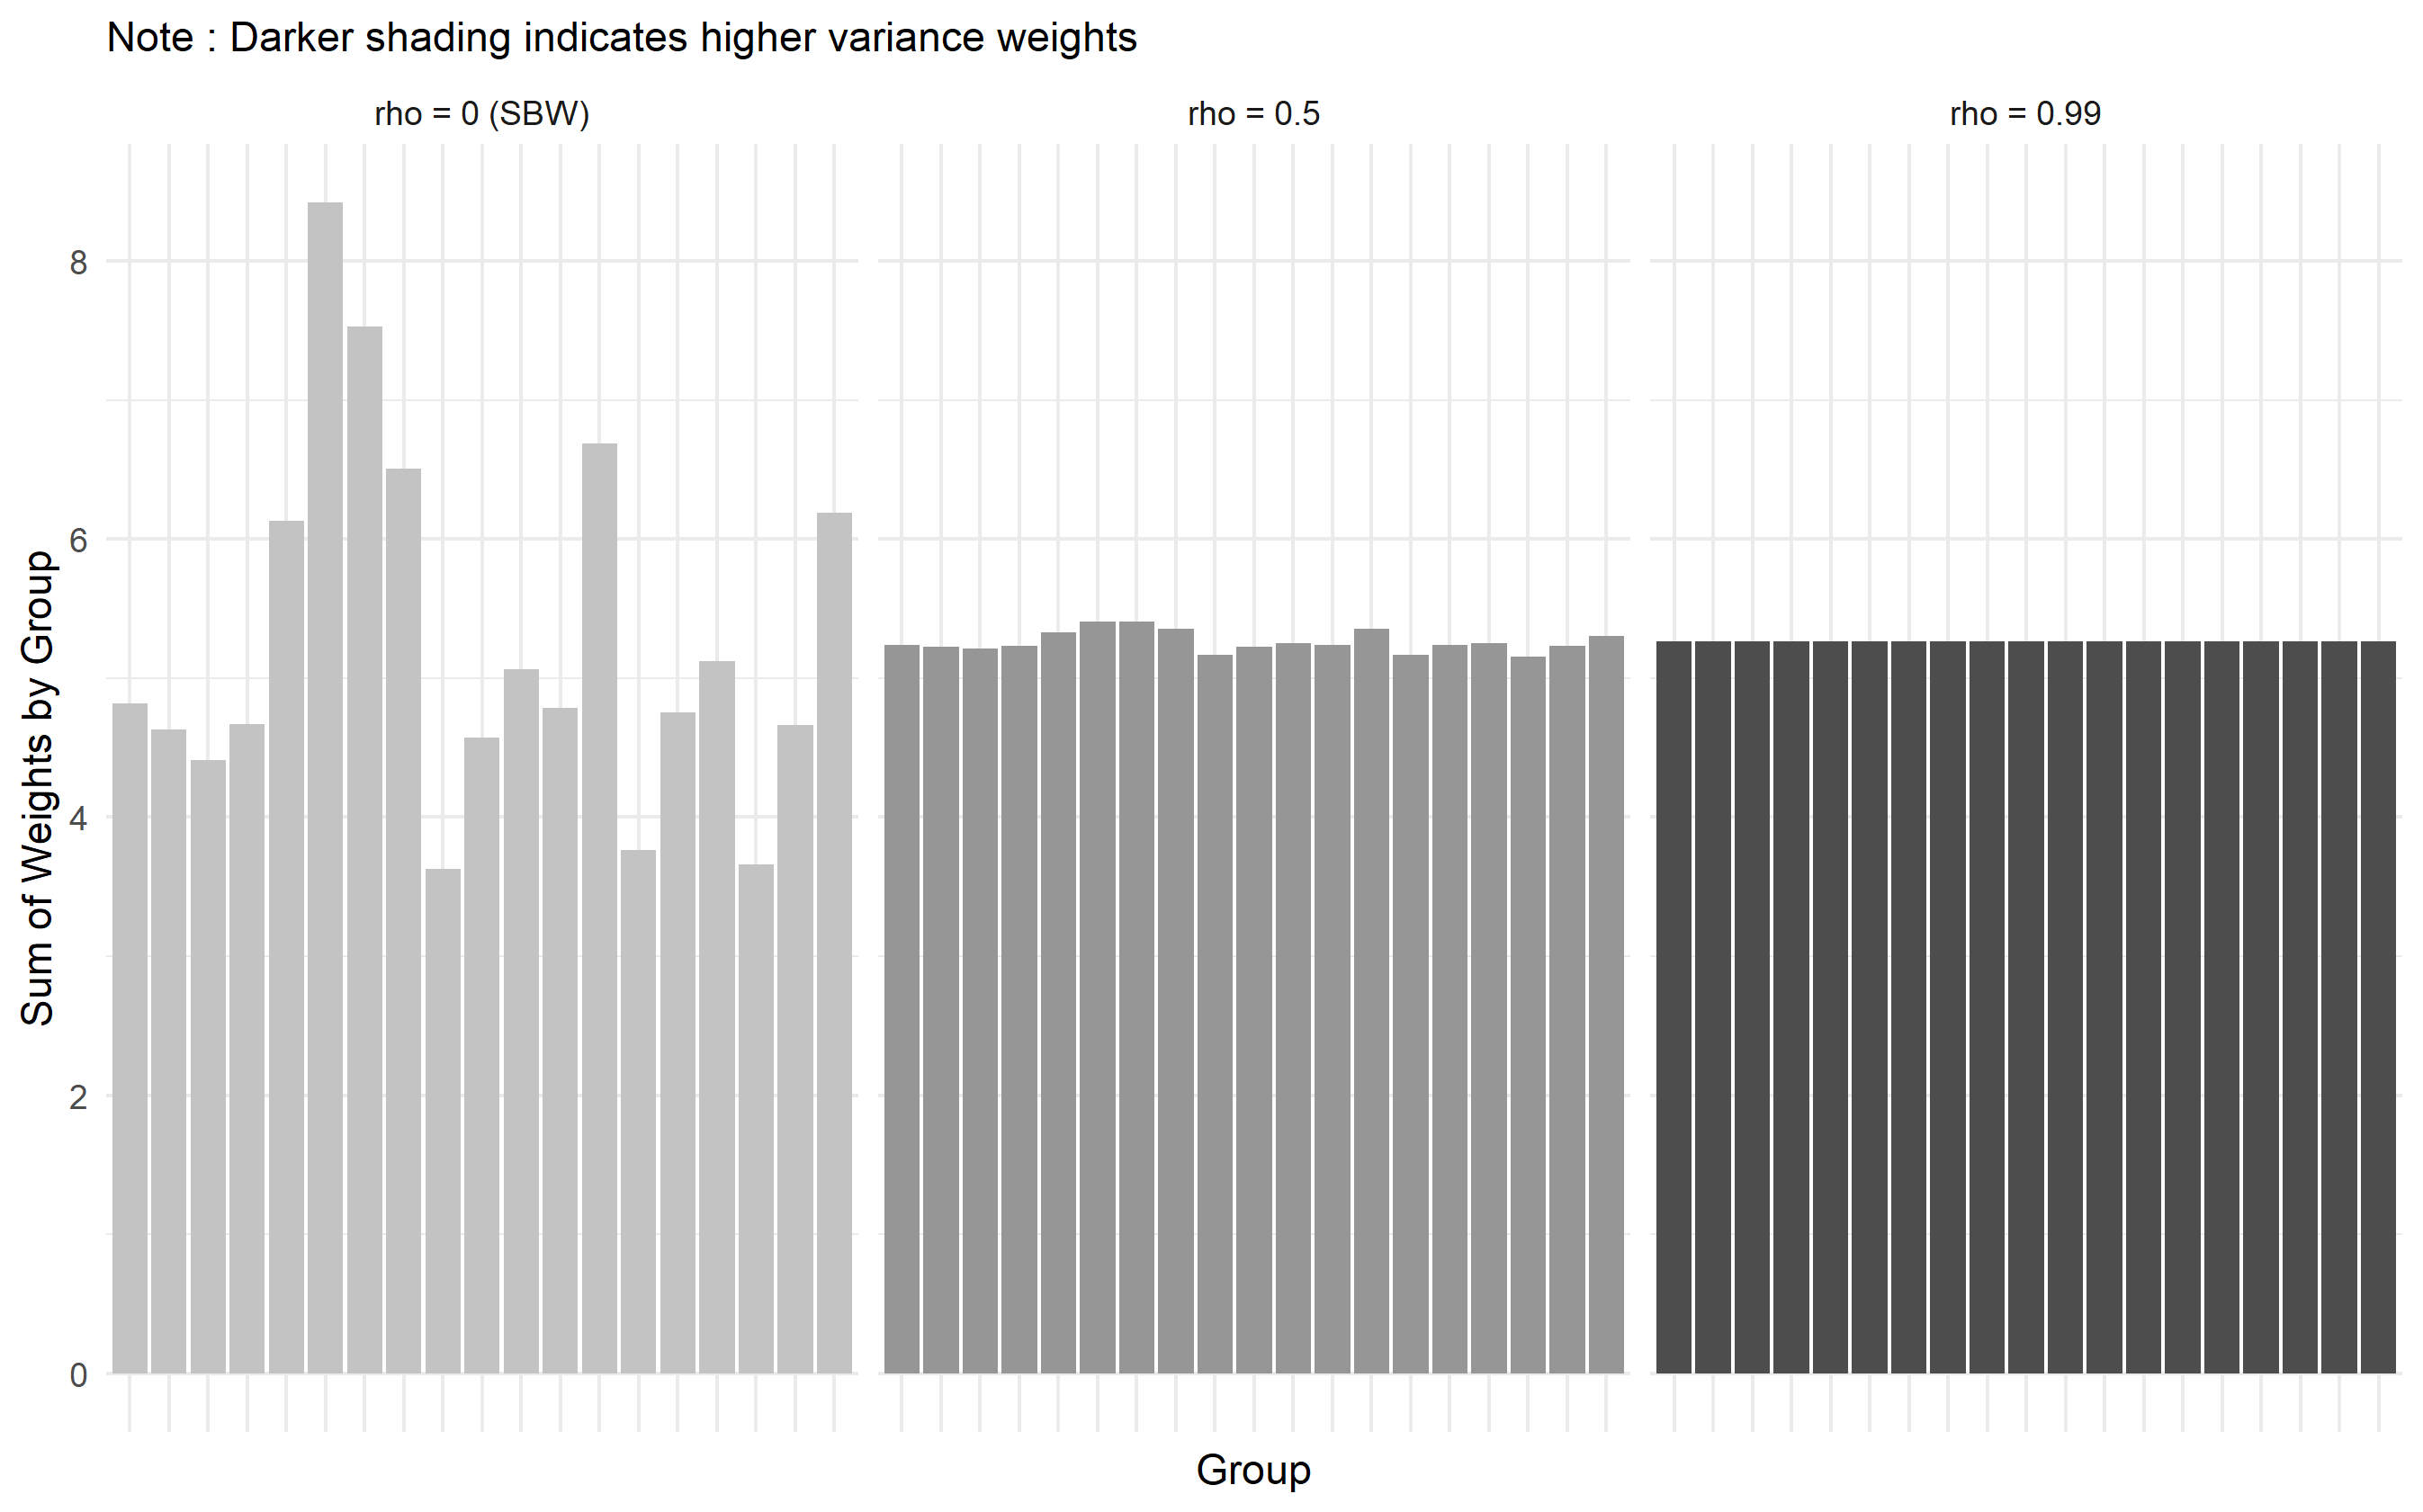
\includegraphics[scale=0.5]{01_Plots/proofofconcept.png}
    \caption{Comparison of SBW and H-SBW: within group sum of weights}
    \label{oatepref}
\end{center}
\end{figure}

The particular covariance structure we assume is identical to the one proposed by \cite{kloek1981ols}. In Appendix A, we show that this objective produces the minimum variance estimator under the constraint set for this correlation structure. We note that theoretically we could incorporate any other assumed covariance structure into this objective, though the number of tuning parameters might change. Broadly speaking, we can think of H-SBW being to SBW what generalized least squares (GLS) is to ordinary least squares (OLS): both SBW and OLS can produce unbiased estimates of model parameters; however, H-SBW and GLS can improve the efficiency of our estimates under different assumed correlation structures of the outcome errors.

\subsubsection{Measurement error}

A second advancement in our estimation procedure comes in our balance constraints: rather than balancing on the observed covariate values $W_{sc}$, we instead balance on the imputed covariate estimates $\hat{\eta}_1(W_{sc})$ (we refer to these as the ``adjusted covariates''). This procedure attempts to correct for the estimation error in these CPUMA-level covariates that may bias our estimate of $\psi^1$. In Appendix A, we consider the super-population target $\psi^{1, sp} = \mathbb{E}\{Y^1 \mid A = 0\}$ and show that under the classical errors-in-variables model, the bias for the SBW estimator that balances on the observed covariates $W$ and sets $\delta = 0$ is equivalent to the bias of a linear combination of coefficient estimates from the OLS-based regression estimator. Specifically, the bias for either estimator is:

\begin{equation}
\mathbb{E}\{\hat{\psi}^{1} - \psi^{1, sp}\} = (\upsilon_0 - \upsilon_1)^T(\kappa - I_d)\beta_1
\end{equation}

The intuition for this result is as follows: exact balancing weights implicitly estimate $\beta_1$ on a subset of the data where we have sufficient covariate overlap. We can therefore think of SBW as returning a solution to some weighted-least squares problem. Assuming that the outcome model holds across all of the data, WLS and OLS are estimating the same $\beta_1$; therefore, the bias that effects the least squares solution will have the same effect on the WLS, and therefore SBW, solution. In Appendix A, Proposition 2, we show that if we had access to $\eta_1$, we can obtain an unbiased estimate of $\psi^{1, sp}$ by reweighting $\eta_1(W_{sc})$.\footnote{For the finite-sample parameter we're targeting, this estimator will have finite-sample bias conditional on $W$ and viewing $X$ as fixed.} Of course, in practice we do not know $\eta_1$ but must instead estimate it using auxillary data. In Appendix A, Proposition 3, we show that we can obtain a consistent of $\psi^{1, sp}$ when balancing on an estimate of $\eta_1$ using auxillary data. 

The key in our application is to estimate $\eta_a$: at a high-level, we use the ACS micro-data replicate survey weights to estimate the covariance matrix of CPUMA sampling-variability $\Sigma_{vv, sc}$. Using our observed data to estimate $\Sigma_{WW \mid A = a}$ and $\bar{W}$, we combine these estimates to generate an estimate of $\eta_a$. This is a technique that comes from the regression-calibration literature (see, e.g., \cite{gleser1992importance}). We also consider an adjustment procedure that further accounts for the differential measurement error due to the highly variable sample sizes used to calculate each covariate. This procedure allows our adjustment to differentially adjust covariate values depending on the sample-sizes involved in the adjustment procedure. We refer to the first procedure the ``homogeneous adjustment'' and the second procedure the ``heterogeneous adjustment'' because the adjustment is constant for all units in the first case, but varies by unit in the second case. Further details about these procedures are available in Appendix B.

This is the first application we are aware of to use regression calibration in the context of balancing weights to address the problem of measurement error. We emphasize two critical assumptions for using this procedure in our context: (1) the outcome model is linear in the true covariates; and (2) the measurement error in the outcome is uncorrelated with the measurement error in the covariates. The first assumption is strong, though often used in practice. The second assumption is reasonable, because our outcomes are estimated from a different cross-section than our covariates. 

\subsubsection{Bias-correction for imbalances}

Because we are unable to reduce the balance constraints to our preferred level without generating very extreme weights, following the recent literature on synthetic controls, we test the sensitivity of our results to the imbalances in the observed (or adjusted) covariates using ridge-regression augmented weights \cite{ben2018augmented}. Letting $\matr{\hat{X}}_1$ be the matrix of adjusted covariates, and $\gamma^{hsbw}$ be our H-SBW weights, we consider the regression-augmented weights:

\begin{equation}
\gamma^{aug} = \gamma^{hsbw} + (\gamma^{hsbw}\hat{X}_1 - \bar{W}_0)^T(\hat{X}_1^T\Omega^{-1}\hat{X}_1 + \lambda I_q)^{-1}\hat{X}_1^T\Omega^{-1}
\end{equation}

where $\Omega$ is a block diagonal matrix with diagonal entries equal to one and the within-group off diagonals equal to $\rho$. We choose $\lambda$ so that the remaining imbalances all fall within 0.5 percentage points. The cost of this procedure is that we must extrapolate off the support of the data, and therefore rely more heavily on our outcome modeling assumptions. We refer to \cite{ben2018augmented} for more details about this procedure. In our results we consider estimators using SBW ($\rho = 0$), H-SBW ($\rho = 1/6$), and ridge-augmented versions of SBW and H-SBW that we call BC-SBW and BC-HSBW. 

\subsection{Model validation}

Earlier we argued that we cannot easily use pre-treatment outcomes to conduct variable selection or to learn about the relative importance of covariates. The challenge with using pre-treatment data in this setting is that it is not obvious why the best model of $\bar{Y}_{0, t}^0$ $(t = T-l,..., T-1)$ should also be the best model, or even a good model, of $\bar{Y}^1_{0,T}$. However, for fixed covariates and targeted levels of imbalance $\delta$, we can use the heuristic that a good model of $\bar{Y}^1_{0,T}$ should also be a good model of $\bar{Y}_{0, t}^0$ to compare our models. We can also assume that when comparing two models, one with uniformly better covariate balance than the other, the model with better covariate balance should have lower bias both for $\bar{Y}_{0, T}^1$ and $\bar{Y}_{0, t}^0$ if our model assumptions are correct. We justify these comparisons by again assuming that $\mu_{a, t}$ are linear in $X$ for all time periods $t$. This is a stronger assumption than we require to estimate the ETC, which only requires that $\mu_{1, T}$ is linear in $X$. However, with this stronger assumption we can use pre-treatment data to at least heuristically compare our models. While we caution that these comparisons may not indicate the best model, we can still use these comparisons to see which models we may trust less.

We therefore rerun our procedures on pre-treatment data to compare the performance of our models for a fixed level of imbalances $\delta$. In particular, we train our model on 2009-2011 data to predict 2012 outcomes, and 2010-2012 data to predict 2013 outcomes. We limit to one-year prediction error since our estimand is only one-year forward. We then examine the performance of the H-SBW versus SBW estimators, which only vary with respect to the tuning parameter $\rho$, the bias-corrected versions, and the covariate adjustment procedure used to determine the weights. 

We expect that the estimators trained on the adjusted data should perform better than the estimators trained on the unadjusted data. If our outcome model is correct, these estimators should achieve better balance across the true covariates and therefore have lower bias than the estimators trained on the unadjusted data. We assume that any difference between the performance of the two adjustments is due to better covariate balance on the true covariates. We therefore use the performance on this data to select which adjustment we prefer in our final results. Conditional on the adjustment, we assume that if the bias-corrected estimators all have uniformly better balance than the uncorrected estimators, these estimators should also perform better than the uncorrected estimators. However, if the assumed outcome models are incorrect, these estimators may suffer from extrapolation bias and perform worse despite achieving better covariate balance. Finally, we expect in general that H-SBW and SBW should have similar performance if we knew the true covariate values. However, in Appendix A, we show that for fixed (unobserved) $X$, these weighting estimators have a finite sample bias that reduces with the square of the weights, suggesting the SBW may have less bias than H-SBW. On the other hand, H-SBW should have less variability given within-state dependencies in the outcomes. From an MSE perspective it is unclear which should be optimal, and given only two-years of pre-treatment data we do not believe we can select which model is better.

\subsection{Inference}

We consider $W$ to be fixed (and $X$ as fixed unknown parameters), and we consider inference over repeated samples from some super-population of CPUMAs with a state-level dependency structure.\footnote{Alternatively, viewing the potential outcomes as fixed and treatment assignment as random, we could consider inference over the randomization distribution of treatment at the state-level.} While placebo tests are frequently used in the synthetic controls literature for inference, we view these as qualitative statistical tests (see, e.g., \cite{arkhangelsky2019synthetic}) and instead use the leave-one-state-out jackknife to estimate the variance of $\hat{\psi}^1$ (\cite{cameron2015practitioner}). Specifically, we exclude each state and re-calculate the weights holding our targeted mean fixed at $\bar{W}_0$.\footnote{When our preferred initial choice of $\delta$ does not converge, we gradually reduce the constraints until it does.} We compute this estimator in two ways: first, we condition on our covariate adjustment $\hat{\eta}_1$. This is our preferred estimator; however, it does not account for the randomness in $\hat{eta}_1$. We therefore also conduct a second procedure where we re-estimate $\hat{\eta}_1$ for each state omitted in the jackknife procedure and provide these results in the Appendix.

To estimate $Var(\hat{\psi}^0 \mid X, W)$ we use an auxillary regression model and use the CR-2 standard error adjustment (using the ``clubSandwich'' package in R) to estimate the variance of the linear combination $\bar{W}_0^T\hat{\beta}_0$. We can estimate this quantity using the original (unadjusted) data given that $\mathbb{E}\{\bar{W}_0^T\hat{\beta}_0\} = \psi^0$ (since the regression line runs through the point $(\bar{W}_0, \bar{J}_0)$, which are unbiased estimates of $(\bar{X}_0, \bar{Y}_0)$). Our total estimate $\hat{Var}(\hat{\psi})$ is simply the sum of these two variance estimates. We use the standard normal quantiles to generate confidence intervals. 
